%%%% Header %%%%%%%%%%%%%%%%%%%%%%%%%%%%%%%%%%%%%%%%%%%%%%%%%%%%%%%%%%%%%%%%%%%

\documentclass[
  12pt
]{scrartcl}

\usepackage{jonas}

\bibliography{/home/jon/lucile/share/jowncloud/sci/refs/refs.bib}
\hyphenation{}

%%%% Meta data %%%%%%%%%%%%%%%%%%%%%%%%%%%%%%%%%%%%%%%%%%%%%%%%%%%%%%%%%%%%%%%%

\usepackage[
  pdfauthor   ={Jonas Schöley},
  pdftitle    ={The Human Mortality Explorer},
  pdfsubject  ={Interactive Visualization},
  pdfkeywords ={visualization, R, shiny, mortality, hmd, Lexis surfaces},
  pdfproducer =Latex,
  pdfcreator  =pdflatex
]{hyperref}

\title{The Human Mortality Explorer}
\subtitle{An Interactive Online Visualization \vskip 0.2em of the Human Mortality Database}
\author{
  Jonas Schöley\footnote{Max-Planck Odense Center on the Biodemography of Aging, University of Southern Denmark. \texttt{jschoeley@health.sdu.dk}}
}

%%%% Titlepage %%%%%%%%%%%%%%%%%%%%%%%%%%%%%%%%%%%%%%%%%%%%%%%%%%%%%%%%%%%%%%%%

\begin{document}

\maketitle

\thispagestyle{empty}

\begin{figure}[ht!]
  \centering
  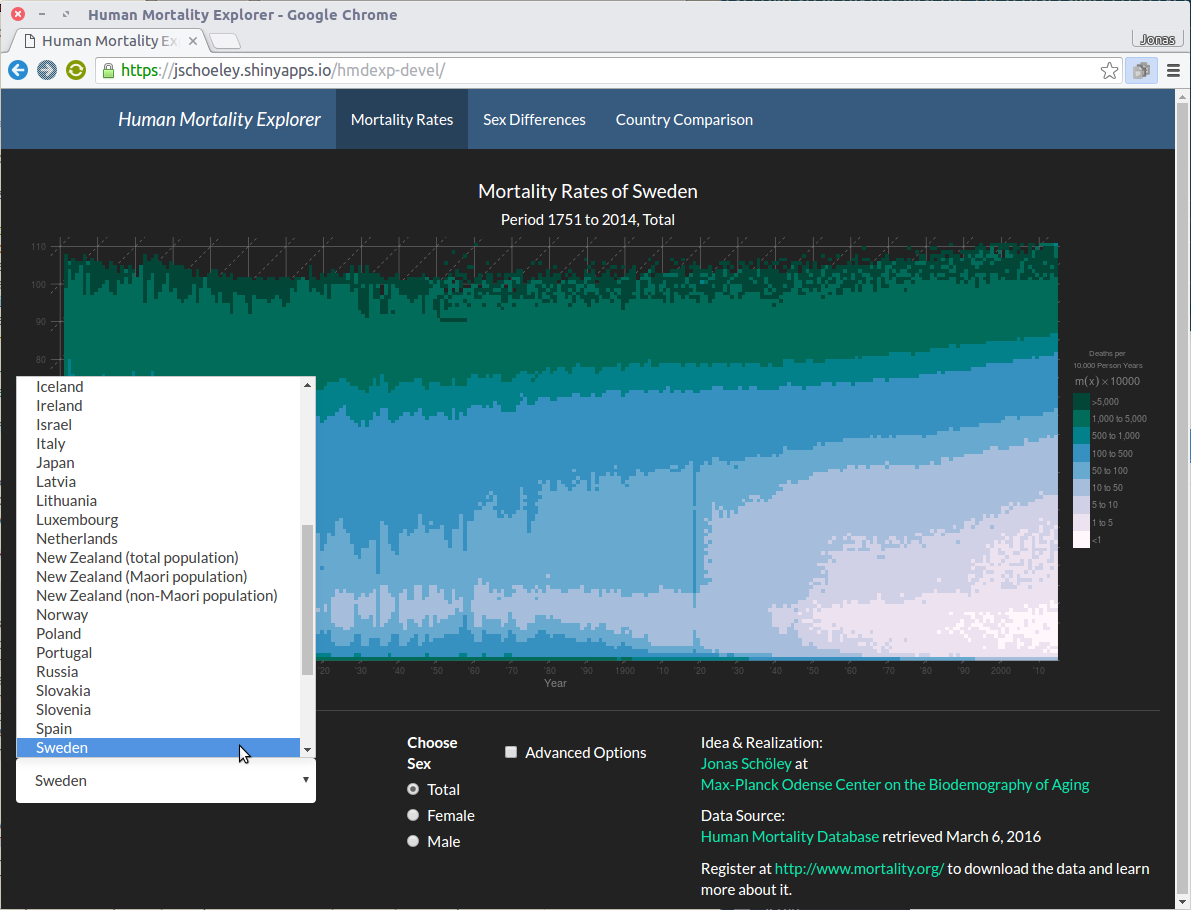
\includegraphics[width = 0.7\textwidth]{./fig/hmd_screen_mx.png}
  \caption*{\textbf{The Human Mortality Explorer:} Mortality surface view.
  \textit{Please visit \url{https://jschoeley.shinyapps.io/hmdexp} to experience the Human Mortality Explorer.}}
\end{figure}

\begin{abstract2}
  The \emph{Human Mortality Explorer} is a web-application for the visual exploration of the Human Mortality Database. It allows anyone with access to the internet to easily explore human mortality dynamics across space and time. Users select data subsets on a graphical user interface and are immediately presented with results in the form of Lexis surface plots (heatmaps over period and age). Users can toggle between a visualization of country specific mortality rates, sex differences in mortality and cross country mortality comparisons. The Human Mortality Explorer is build using modern technologies that facilitate the rapid construction of interactive web-pages without requiring expert knowledge on web-technologies. It showcases the utility of web-applications as part of a demographers toolbox.
\end{abstract2}

\clearpage

%%%% Text %%%%%%%%%%%%%%%%%%%%%%%%%%%%%%%%%%%%%%%%%%%%%%%%%%%%%%%%%%%%%%%%%%%%%

\section*{Background}

Interactive visualizations hosted on the web are the medium of many success stories in recent years. \emph{\enquote{The Global Flow of People}} (\cite{Sander2014}), \emph{\enquote{Gapminder World}} (\cite{Rosling2006}) or \emph{\enquote{What's Really Warming the World?}} (\cite{Roston2015}) are examples of visualizations able to generate publicity and to engage people in the subject matter. Less visible but of equal importance are domain specific visualization tools which help scientists with specific data analysis tasks such as genome analysis (\emph{\enquote{MizBee}}, \cite{Meyer2009}), cluster analysis (\emph{\enquote{Hierarchical Clustering Explorer}}, \cite{Seo2002}), browsing linguistic networks (\emph{\enquote{Constellation}}, \cite{Munzner1999}), poetry analysis (\emph{\enquote{RhymeDesign}}, \cite{McCurdy2015}) or investigative journalism (\emph{\enquote{RevEx}}, \cite{Bertini2015}), to name a few.

Today the barrier of entry for building such applications is lower than ever and researchers can build web-applications themselves without relying on external expertise. The \emph{Human Mortality Explorer}, a web-based tool designed for easy exploration of the popular Human Mortality Database (\cite{Hmd2016}), serves to demonstrate this point. It has been developed over the course of a month by a single researcher.

\section*{Objective}

The objective is to develop a tool that allows for the \emph{easy and quick exploration of data on human mortality} by researchers, teachers, students and the interested public. Researchers should be able to quickly check existing hypotheses against the data and generate new ones. Teachers are given a tool to effortlessly illustrate classes on human mortality patterns while at the same time being able to explore the HMD data together with their students, facilitating classroom interactions. The interested public enjoys easy access to demographic data on international mortality. In order to reach such a wide and heterogeneous audience the tool has to be \emph{available online}, must be \emph{easy-to-use} and \emph{stable}.

\section*{Methods}

The application is written in the \texttt{R} language for statistical computing (\cite{RCT2016}). The \texttt{shiny} library (\cite{Chang2016}) is used to build a web-based user interface from within \texttt{R}. A special web server capable of interpreting \texttt{R + shiny} code hosts the application. The choice of tools illustrates an important point: Nowadays web-applications can be build by a single researcher, in a known programming environment, without deep knowledge about \texttt{HTML}, \texttt{Java Script} or other web technologies. Development takes place in the open. The source code is publicly available at an online repository (\url{https://github.com/jschoeley/hmdexp/}).

\section*{Contribution}

The \emph{Human Mortality Explorer} is a web-application for the visual exploration of the Human Mortality Database, showing mortality-rates across time and space. The tool is available to anyone connected to the internet. \textbf{A Demonstration:}

\begin{figure}[ht!]\centering
  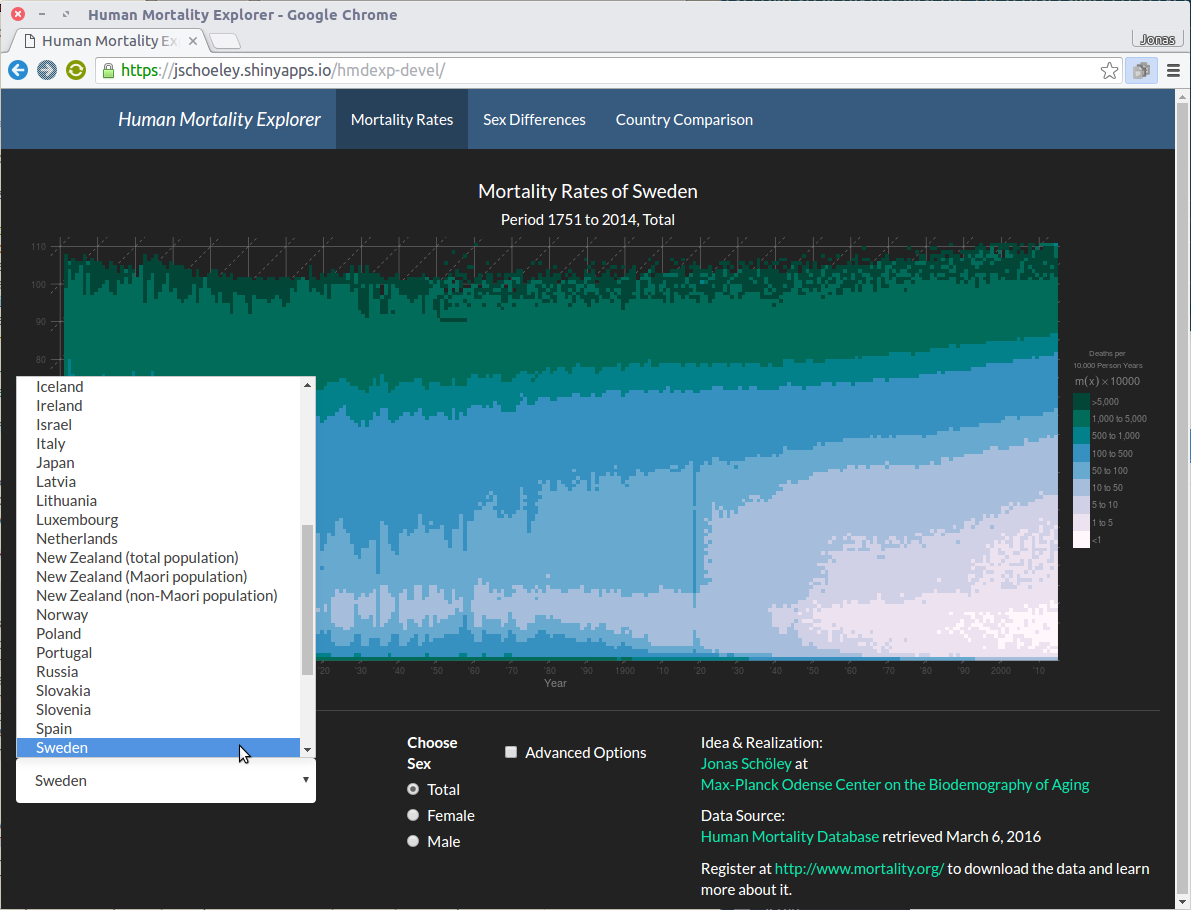
\includegraphics[width = \linewidth]{./fig/hmd_screen_mx.png}
  \caption*{\textbf{First steps:} Users are greeted with a Lexis surface view of Swedish mortality rates. They are invited to select a different country or a different sex. Further settings are hidden behind an \enquote{Advanced Options} check-box in order to make the initial experience as straightforward as possible.}
  \label{fig:mx}
\end{figure}

\begin{figure}[ht!]\centering
  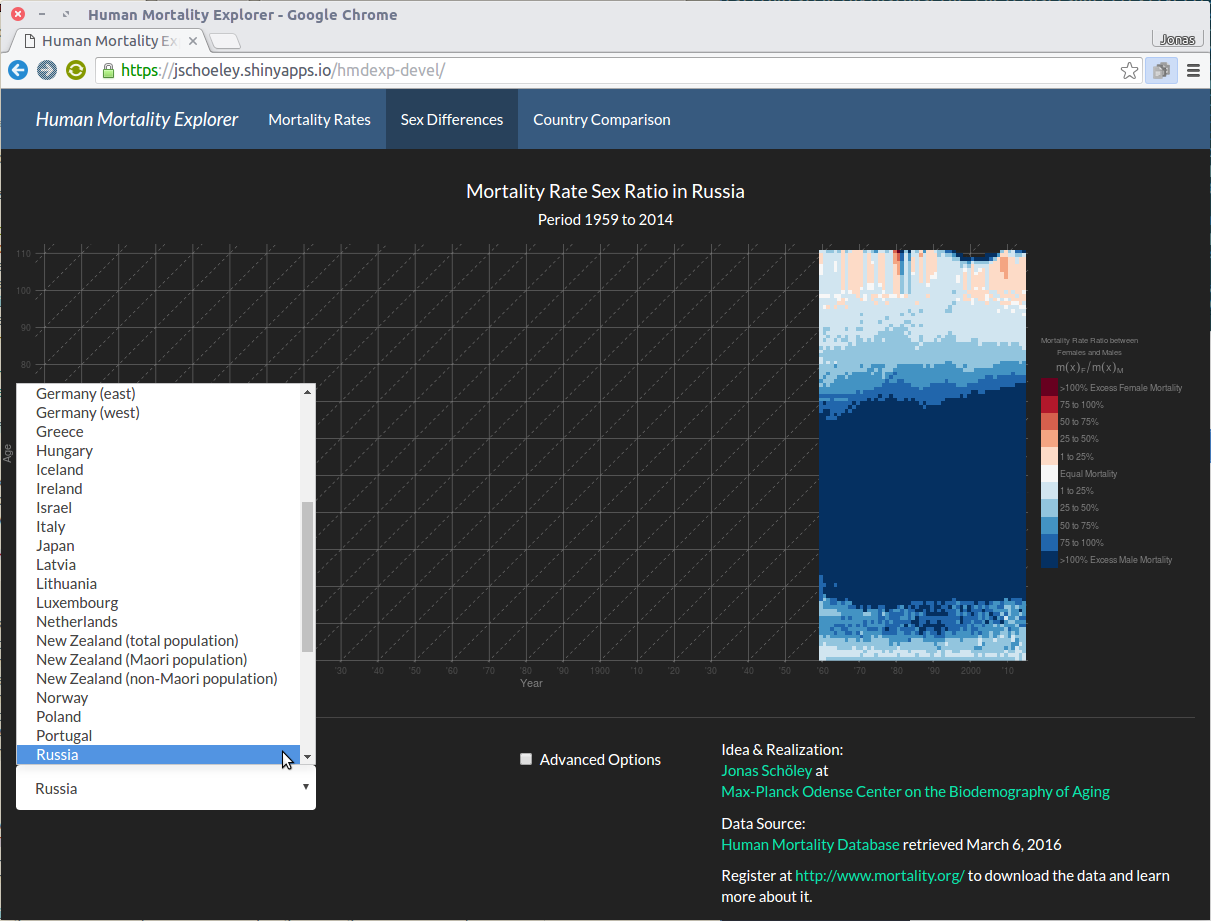
\includegraphics[width = \linewidth]{./fig/hmd_screen_mx_sex_diff.png}
  \caption*{\textbf{Sex differences:} The sex differences view shows the female-male sex ratio of mortality rates for a selected country by period and age. Red areas show excess female mortality, blue areas excess male mortality. Note that the title of the plot always gives information about the measure, the country, and the length of the time series.}
  \label{fig:mx_sex_diff}
\end{figure}

\begin{figure}[ht!]\centering
  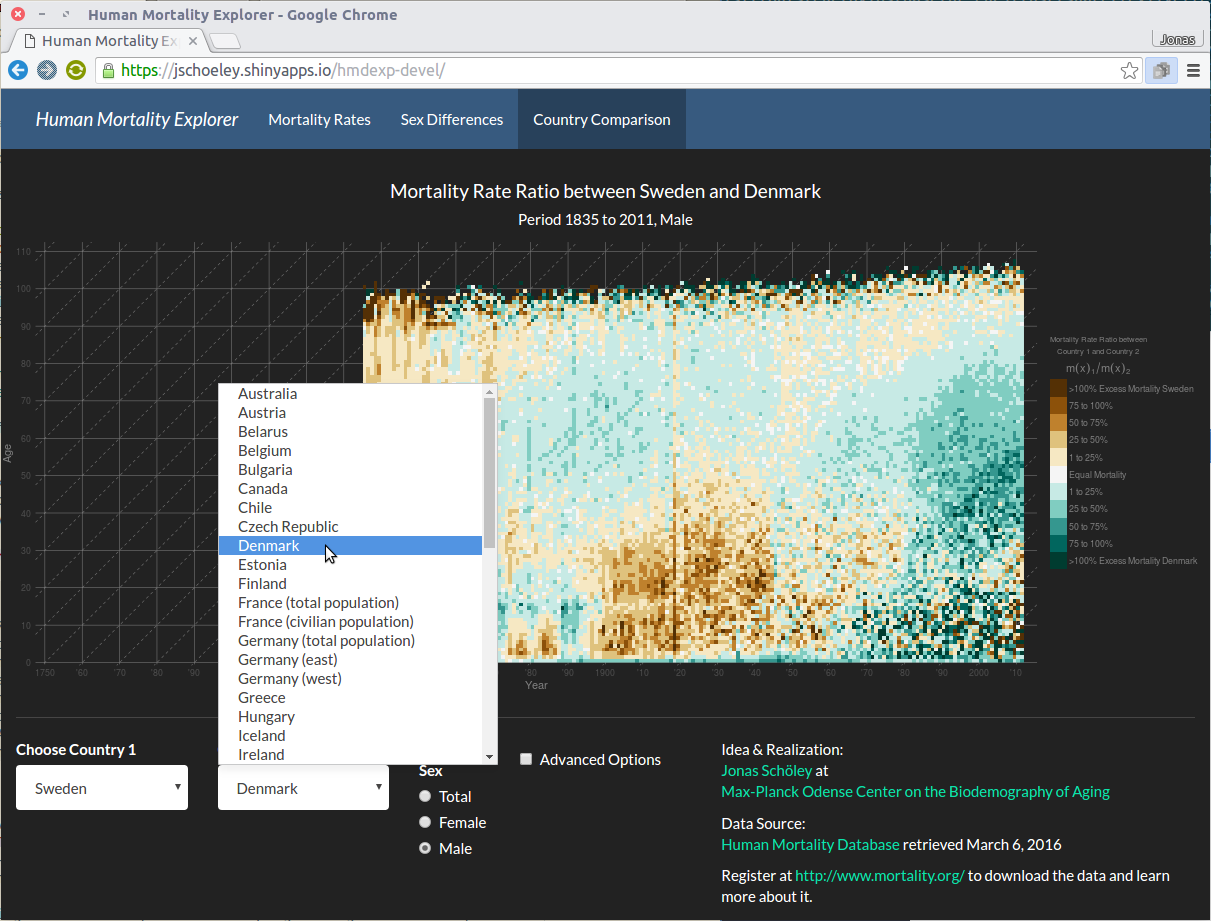
\includegraphics[width = \linewidth]{./fig/hmd_screen_mx_cntry_diff.png}
  \caption*{\textbf{Country differences:} The country differences view works similar to the sex differences view. Users select two countries two compare with each other and are then presented with the mortality rate ratios of both countries in form of a Lexis surface plot. Note that the colour legend automatically updates itself with the corresponding country names.}
  \label{fig:mx_cntry_diff}
\end{figure}

\begin{figure}[!htb]
  \begin{subfigure}[t]{0.5\textwidth}
    \centering
    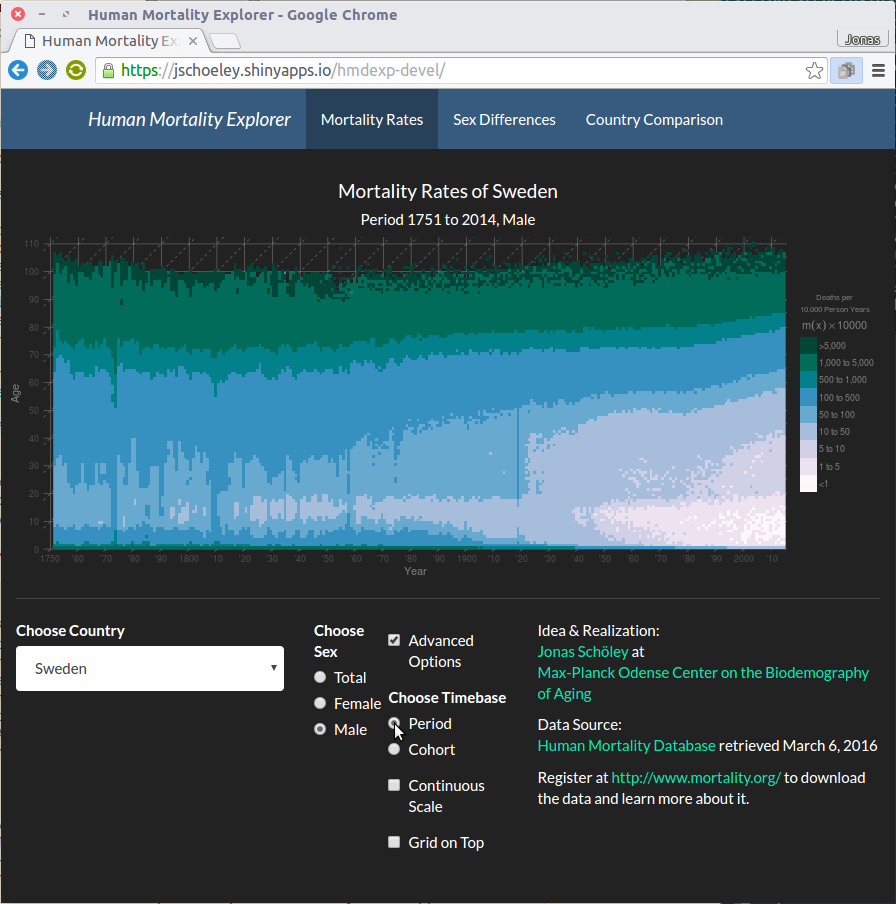
\includegraphics[width = \textwidth]{./fig/hmd_screen_period.png}
    \subcaption*{Showing period mortality rates.}
    \label{fig:mx_period}
    \end{subfigure}%
  ~
    \begin{subfigure}[t]{0.5\textwidth}
    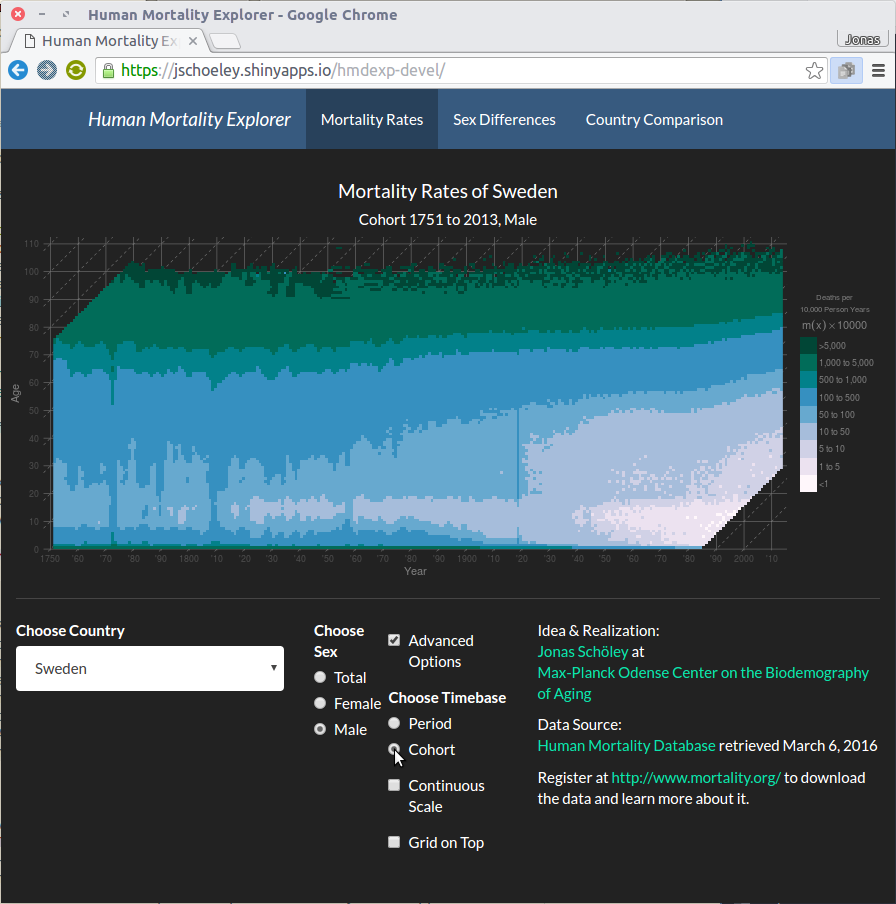
\includegraphics[width = \textwidth]{./fig/hmd_screen_cohort.png}
    \subcaption*{Showing cohort mortality rates.}
    \label{fig:mx_cohort}
    \end{subfigure}%
    \caption*{\textbf{Period and cohort rates:} Users can choose between period- and cohort mortality rates. The cohort rates are projected onto the period-age Lexis grid so that cohorts appear as 45 degree diagonals.}
    \label{fig:mx_pc}
\end{figure}

\begin{figure}[!htb]
  \begin{subfigure}[t]{0.5\textwidth}
    \centering
    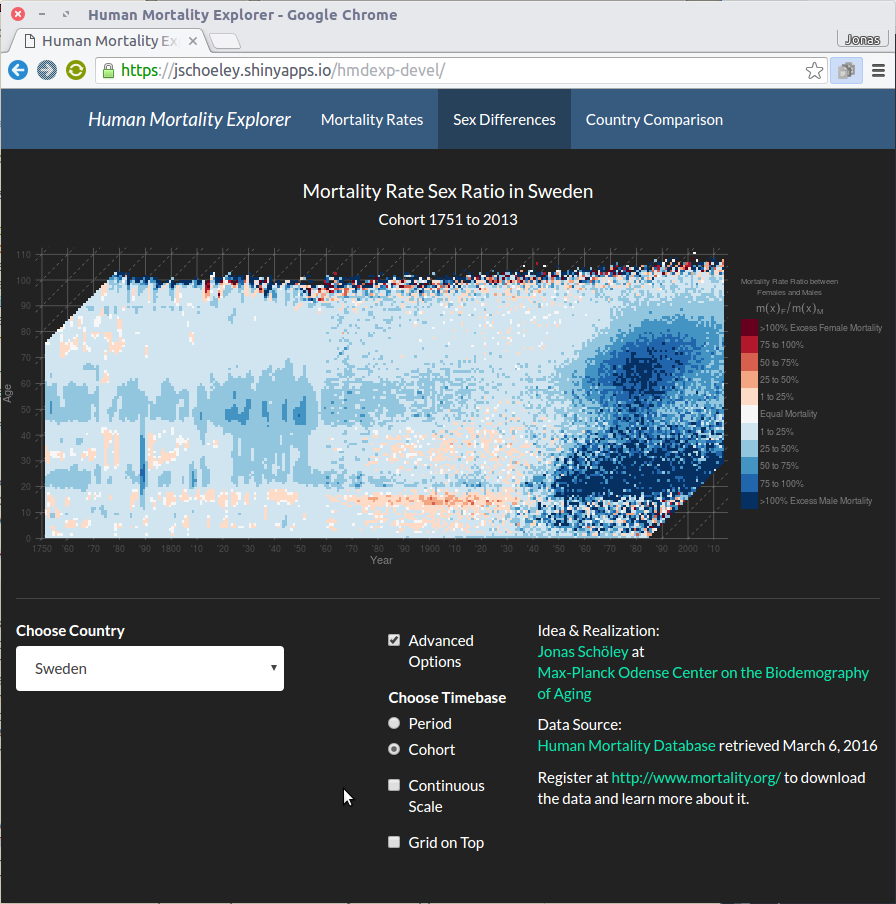
\includegraphics[width = \textwidth]{./fig/hmd_screen_disc_col.png}
    \subcaption*{Using a discrete colour scale.}
    \label{fig:mx_disc}
    \end{subfigure}%
  ~
    \begin{subfigure}[t]{0.5\textwidth}
    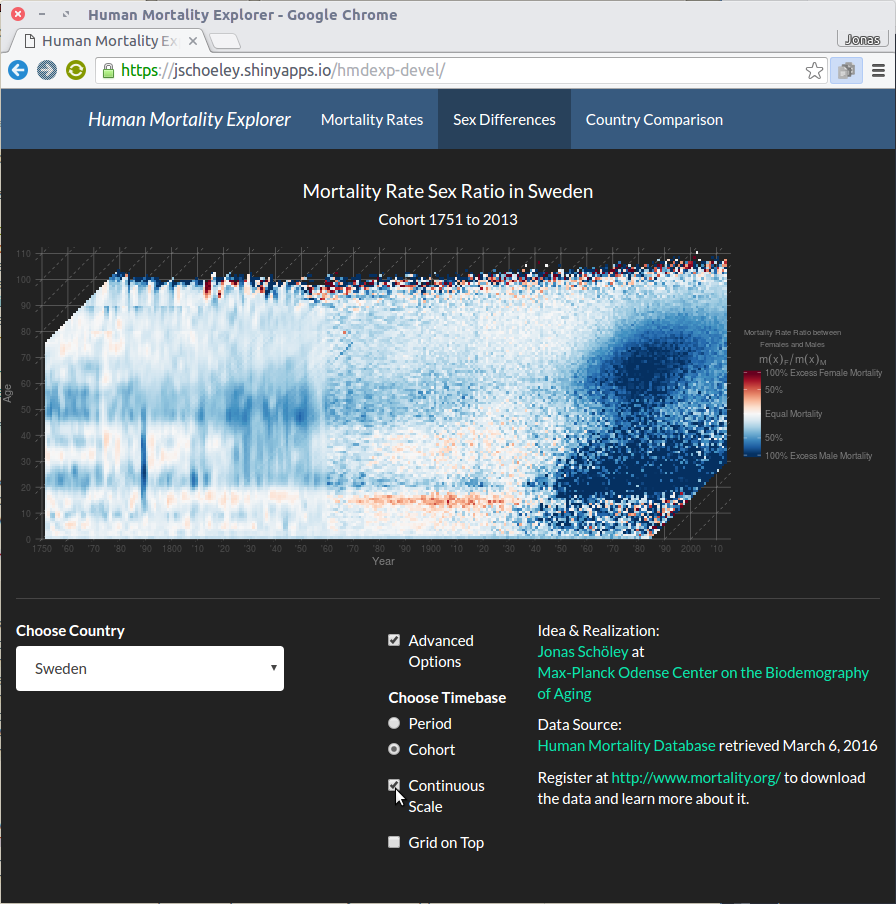
\includegraphics[width = \textwidth]{./fig/hmd_screen_cont_col.png}
    \subcaption*{Using a continuous colour scale.}
    \label{fig:mx_cont}
    \end{subfigure}%
    \caption*{\textbf{Discrete and continuous colour scales:} Users can choose between discrete- and continuous colour scales. The discrete scale is the default as the hard contours facilitate the identification of global patterns. With the continuous colour scale however all information is retained as no binning takes place.}
    \label{fig:mx_scales}
\end{figure}

\begin{figure}[!htb]
  \begin{subfigure}[t]{0.5\textwidth}
    \centering
    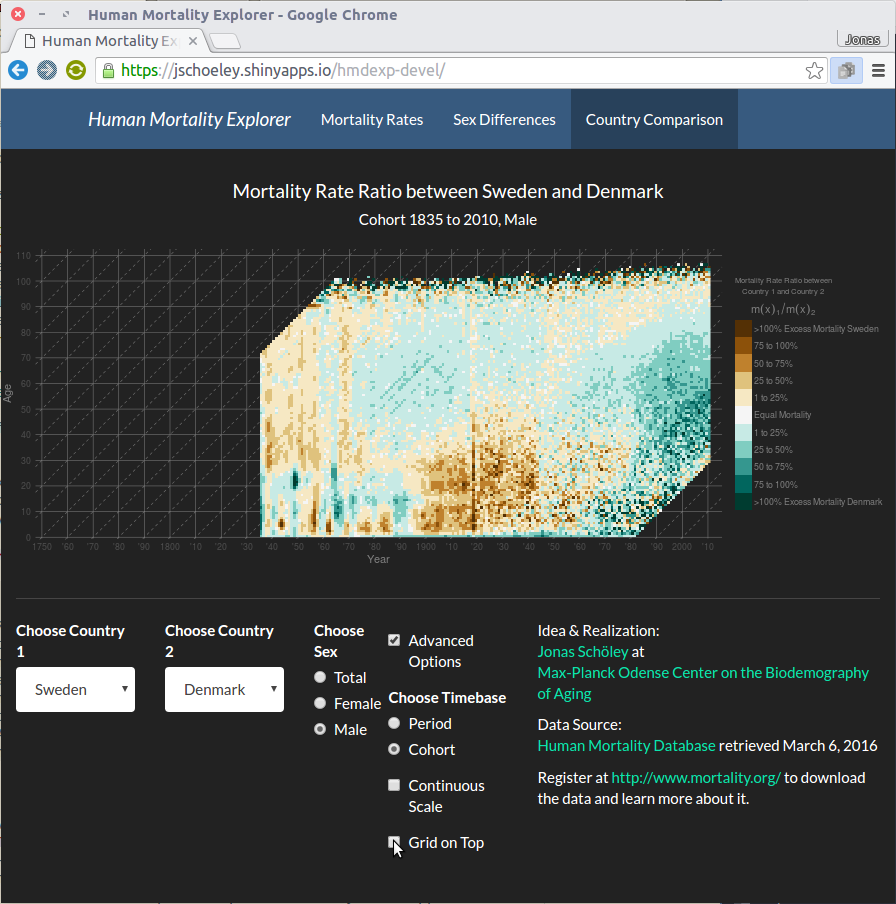
\includegraphics[width = \textwidth]{./fig/hmd_screen_grid_below.png}
    \subcaption*{Grid lines underneath the data.}
    \label{fig:mx_grid_below}
    \end{subfigure}%
  ~
    \begin{subfigure}[t]{0.5\textwidth}
    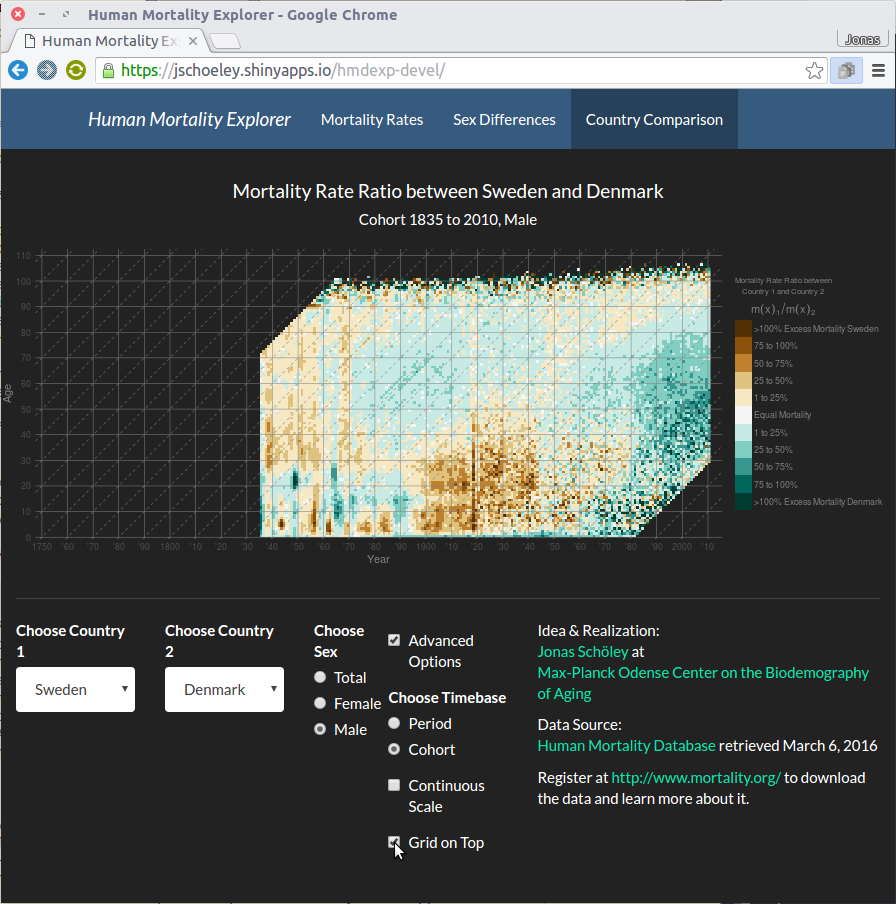
\includegraphics[width = \textwidth]{./fig/hmd_screen_grid_above.png}
    \subcaption*{Grid lines on top of the data.}
    \label{fig:mx_grid_above}
    \end{subfigure}%
    \caption*{\textbf{Positioning of grid-lines:} The grid-lines for period, age, and cohort can be put underneath the data (default) or on top of it.}
    \label{fig:mx_grid}
\end{figure}

\begin{figure}[!htb]
  \begin{subfigure}[t]{0.5\textwidth}
    \centering
    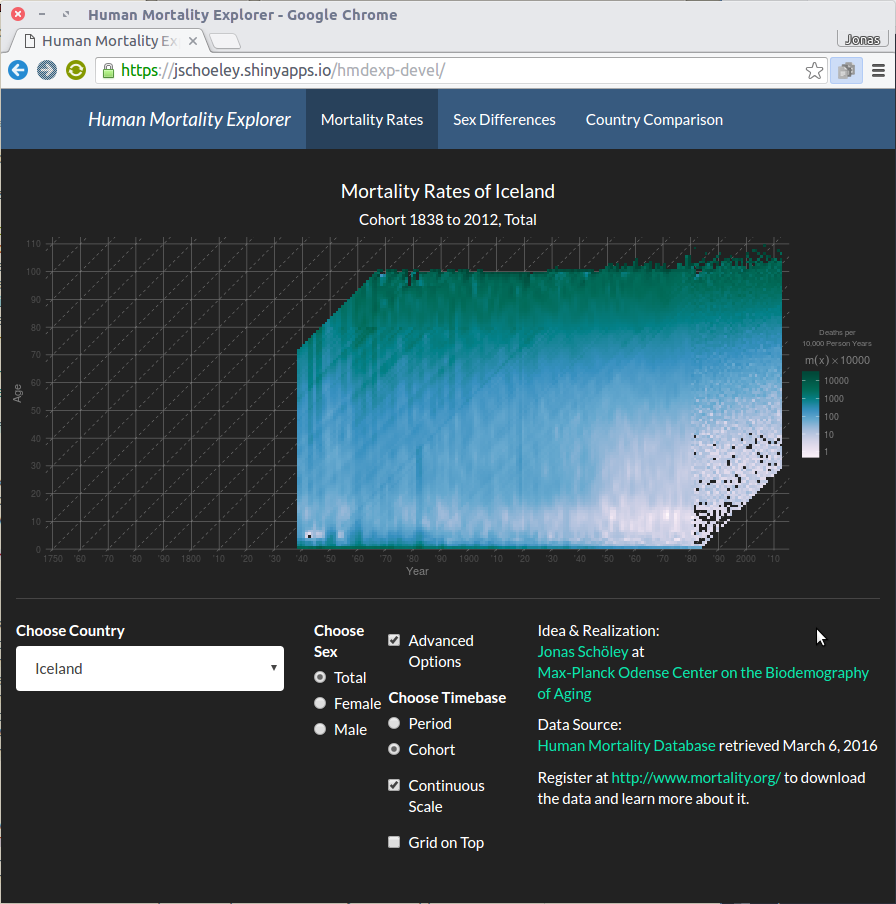
\includegraphics[width = \textwidth]{./fig/hmd_screen_wide.png}
    \subcaption*{The Human Mortality Explorer as seen on a laptop.}
    \label{fig:mx_wide}
    \end{subfigure}%
  ~
    \begin{subfigure}[t]{0.5\textwidth}
    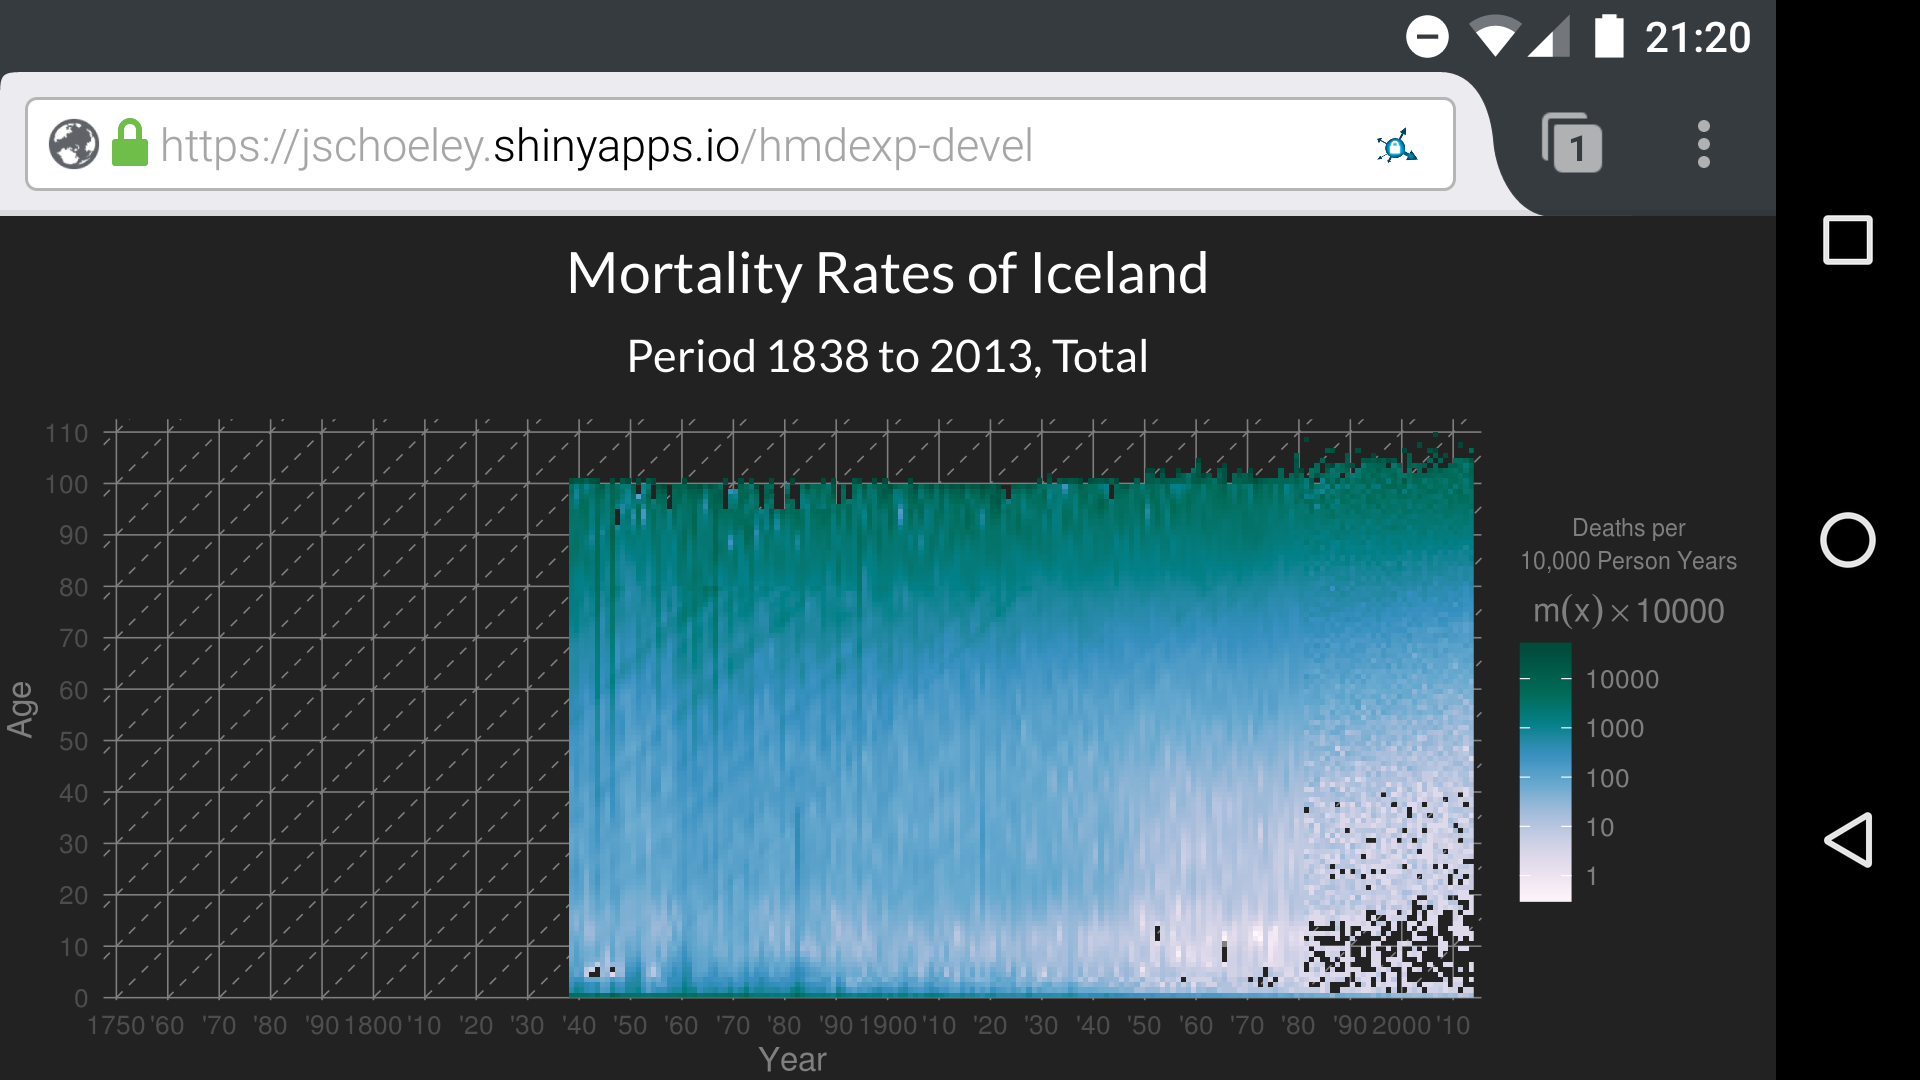
\includegraphics[width = \textwidth]{./fig/hmd_screen_phone.png}
    \subcaption*{The Human Mortality Explorer as seen on a smartphone.}
    \label{fig:mx_long}
    \end{subfigure}%
    \caption*{\textbf{Available on all devices:} The application can be used with any device that supports modern web-browsers such as classical desktop computers, laptops or mobile devices like tablets and smartphones. The user-interface is automatically scaled according to the screen size of the display device.}
    \label{fig:size}
\end{figure}

\clearpage

%%%% Bibliography %%%%%%%%%%%%%%%%%%%%%%%%%%%%%%%%%%%%%%%%%%%%%%%%%%%%%%%%%%%%%

\sloppy
\printbibliography

%\clearpage

%%%% Appendix %%%%%%%%%%%%%%%%%%%%%%%%%%%%%%%%%%%%%%%%%%%%%%%%%%%%%%%%%%%%%%%%%

% appendix figures follow A1, A2, B1... scheme
%\renewcommand\thefigure{\thesection.\arabic{figure}}
%\setcounter{figure}{0}

%\begin{appendix}
%\end{appendix}

\end{document}